% 2011 年福建卷文科第 20 题：四棱锥 P-ABCD，PA⊥底面，CE∥AB。
% 来源 PDF：普通高考/2011/2011福建文.pdf，SHA-256 e649bdc736a215d4e41e02c6a7945953aca84a87a23e6a903596d61025cdf322。
% 原页：第 2 页第 1 栏下部，书页码 662。示意。
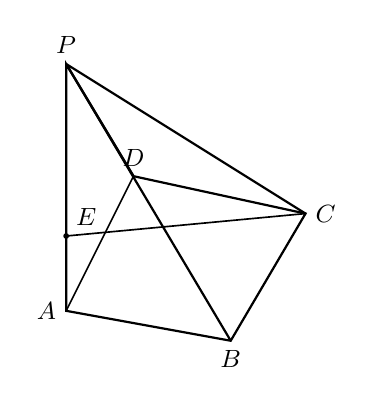
\begin{tikzpicture}[>=stealth, semithick, font=\small, scale=0.95]
  \coordinate (A) at (0,0);
  \coordinate (B) at (2.2,-0.4);
  \coordinate (D) at (0.9,1.8);
  \coordinate (C) at (3.2,1.3);
  \coordinate (E) at (0,1.0);
  \coordinate (P) at (0,3.3);
  \draw[thick] (P)--(A)--(B)--(C)--(D)--cycle;
  \draw[thick] (P)--(B) (P)--(C) (P)--(D);
  \draw (A)--(D);
  \draw (C)--(E);
  \fill (E) circle (1.1pt) node[above right] {$E$};
  \node[left] at (A) {$A$}; \node[below] at (B) {$B$};
  \node[right] at (C) {$C$}; \node[above] at (D) {$D$};
  \node[above] at (P) {$P$};
\end{tikzpicture}
